\section{Erlang Subsystem}\label{sec:erlang_subsystem}

The Erlang Subsystem manages the persistence of auctions and bids data and is
responsible for the calculation is responsible for calculating the auction
status. The Erlang Subsystem is designed and implemented with techniques that
allow availability and fault tollerance. The Erlang Subsystem takes advantage of
Erlang language and Erlang's runtime system and its concurrent computing
capabilities.

\figref{fig:erlang_arch} shows the Erlang Subsystem's logical architecture.

\begin{figure}[h]
	\centering
	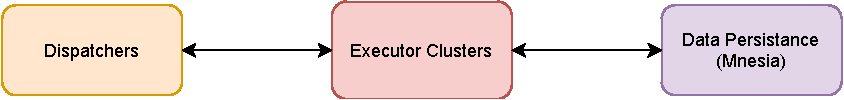
\includegraphics[width=\textwidth]{erlang_arch}
	\caption{Erlang Subsystem logical architecture}\label{fig:erlang_arch}
\end{figure}

\subsection{Dispatchers}

Dispatchers are a set of erlang processes which have the task of interfacing
with the application server. The task of a dispatcher is to assign the
management of an auction to a cluster executor when an auction creation request
arrives from the application server and subsequently forward the requests for
that auction to the same executor cluster. The assignment of the auction to the
cluster is done through a calculation between the id of the auction and the id
of the cluster, for this reason every dispatcher knows where to forward the
requests without the need for any kind of communication between them. Whenever
the application server has a request for the erlang subsystem, it sends it to a
dispatcher which will forward the request to the cluster executor managing that
auction. Once the response from the cluster executor is received, the dispatcher
will forward the response to the application server. Dispatchers are implemented
through the \textit{gen\_server} behavior.

\subsection{Executor Clusters}

The executor clusters are a set of cluster and each cluster is composed of a set
of erlang processes. The choice for which it was decided to implement a cluster
structure will be described in the section Fault Tollerance Techiques. Each
executor cluster manages a subset of auctions of the system (the assignment of
an auction to a cluster is decided, as previously mentioned, by the
dispatchers). Each cluster communicates with Mnesia (we will see later) for the
data persistence and manages the progress of the auctions for which it is
responsible. In particular, for each auction, the cluster must calculate the
so-called \textbf{AuctionState}, \idest*{produce the list of current winning
bids each time a bid is added or deleted}.


Following the \underline{all-or-nothing} semantics described in the
specifications, the \textbf{AuctionState} is calculated by taking the bids with
the highest value (for the same value, the oldest bid is considered as the best)
and that the sum of the quantities of items requested by these is less than or
equal to the quantity of items for sale. Furthermore, it is ensured that only
one bid per user is among the winning ones.

\figref{fig:auction_state_example} shows an AuctionState computation example.

%ADD EXAMPLE IMAGE

\begin{figure}[h]
	\centering
	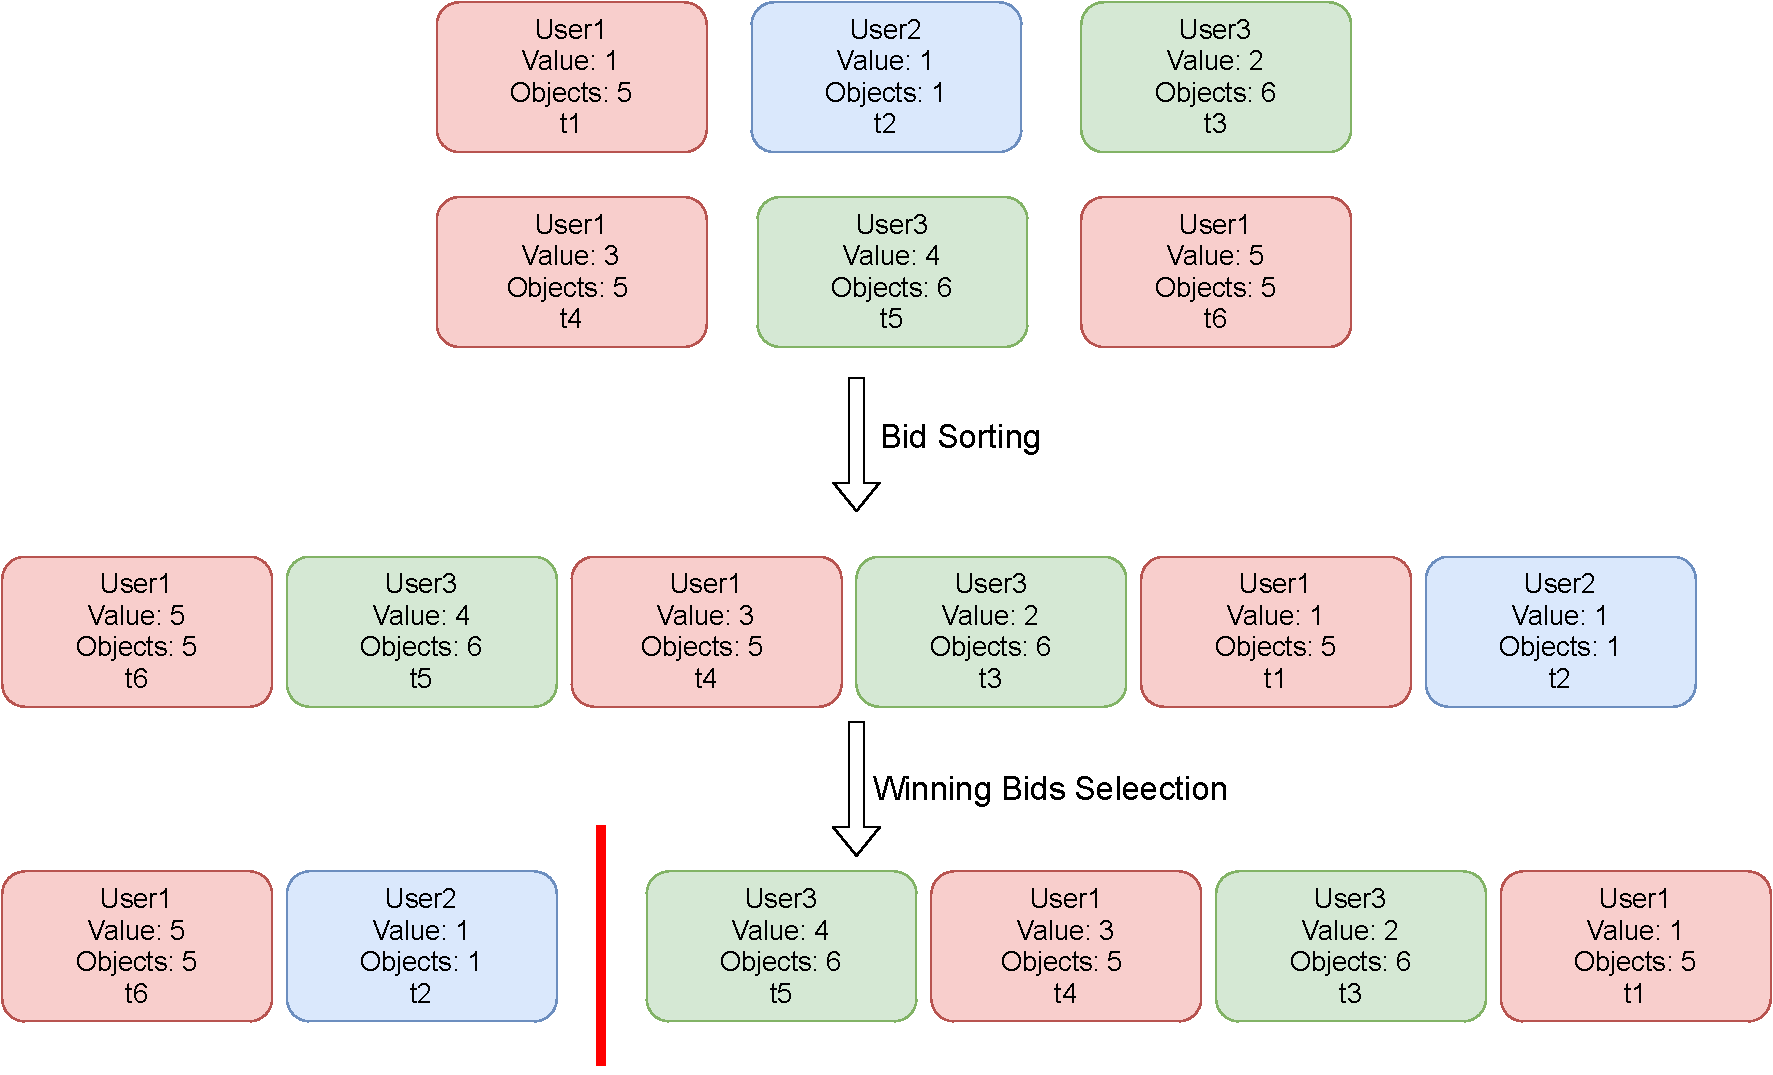
\includegraphics[width=\textwidth]{auction_state_example}
	\caption{AuctionState Computation}\label{fig:auction_state_example}
\end{figure}

The AuctionState is kept in memory in order to be sent upon request by the
application server and is recalculated (and subsequently sent) every time an
offer is added or deleted. Executor processes are implemented through the
\textit{gen\_server} behavior.



\subsection{Data Persistance --- Mnesia}

The persistence of data (auctions and bids) is managed by Mnesia, a distributed
telecommunications DBMS that allows persistence, data replication, atomic
transactions, and location transparency.

For the persistence of auctions and bids, two tables of type \textit{set} have
been created on Mnesia. To define the attributes of the tables, the following
records been defined.


\begin{lstlisting}[language=Erlang, caption=Mnesia Record]
    -record(auction,{%
        id_auction, 
        id_agent, 
        name, 
        image, 
        description, 
        end_date, 
        min_price, 
        min_raise, 
        sale_quantity
    }).
    
    -record(bid, {%
        id_bid, 
        id_auction, 
        id_user, 
        timestamp,
        bid_value, 
        quantity
    }).
\end{lstlisting}


Through a specific Erlang module the following methods have been defined to
interact with Mnesia. All the operations inside the methods have been
implemented through \textit{mnesia:transaction} which allows to perform
transactional operations on Mnesia.


\begin{description}
    \item [insert\_auction]: insert the auction passed as value;
    \item [insert\_bid]: insert the bid passed as value;
    \item [delete\_auction]: delete the auction with the id passed as value;
    \item [delete\_bid]: delete the bid with the id passed as value;
    \item [get\_auction]: returns a specific auction;
    \item [get\_bid\_list]: returns the list of bids for an auction (and
	    optionally, of a given user);
    \item [get\_auction\_list]: returns the list of auctions available;
    \item [get\_bidder\_auctions]: returns the list of auctions in which the
	    user has made at least 1 bid;
    \item [get\_agent\_auctions]: returns the list of auctions created by an
	    agent
\end{description}


\subsection{Fault Tollerance Techinques}
For each module of the Erlang Susbystem some techniques have been implemented to
ensure a good degree of availability and tolerance to tastes.

\figref{fig:erlang_arch2} shows the Erlang Subsystem's architecture.

\begin{figure}[H]
	\centering
	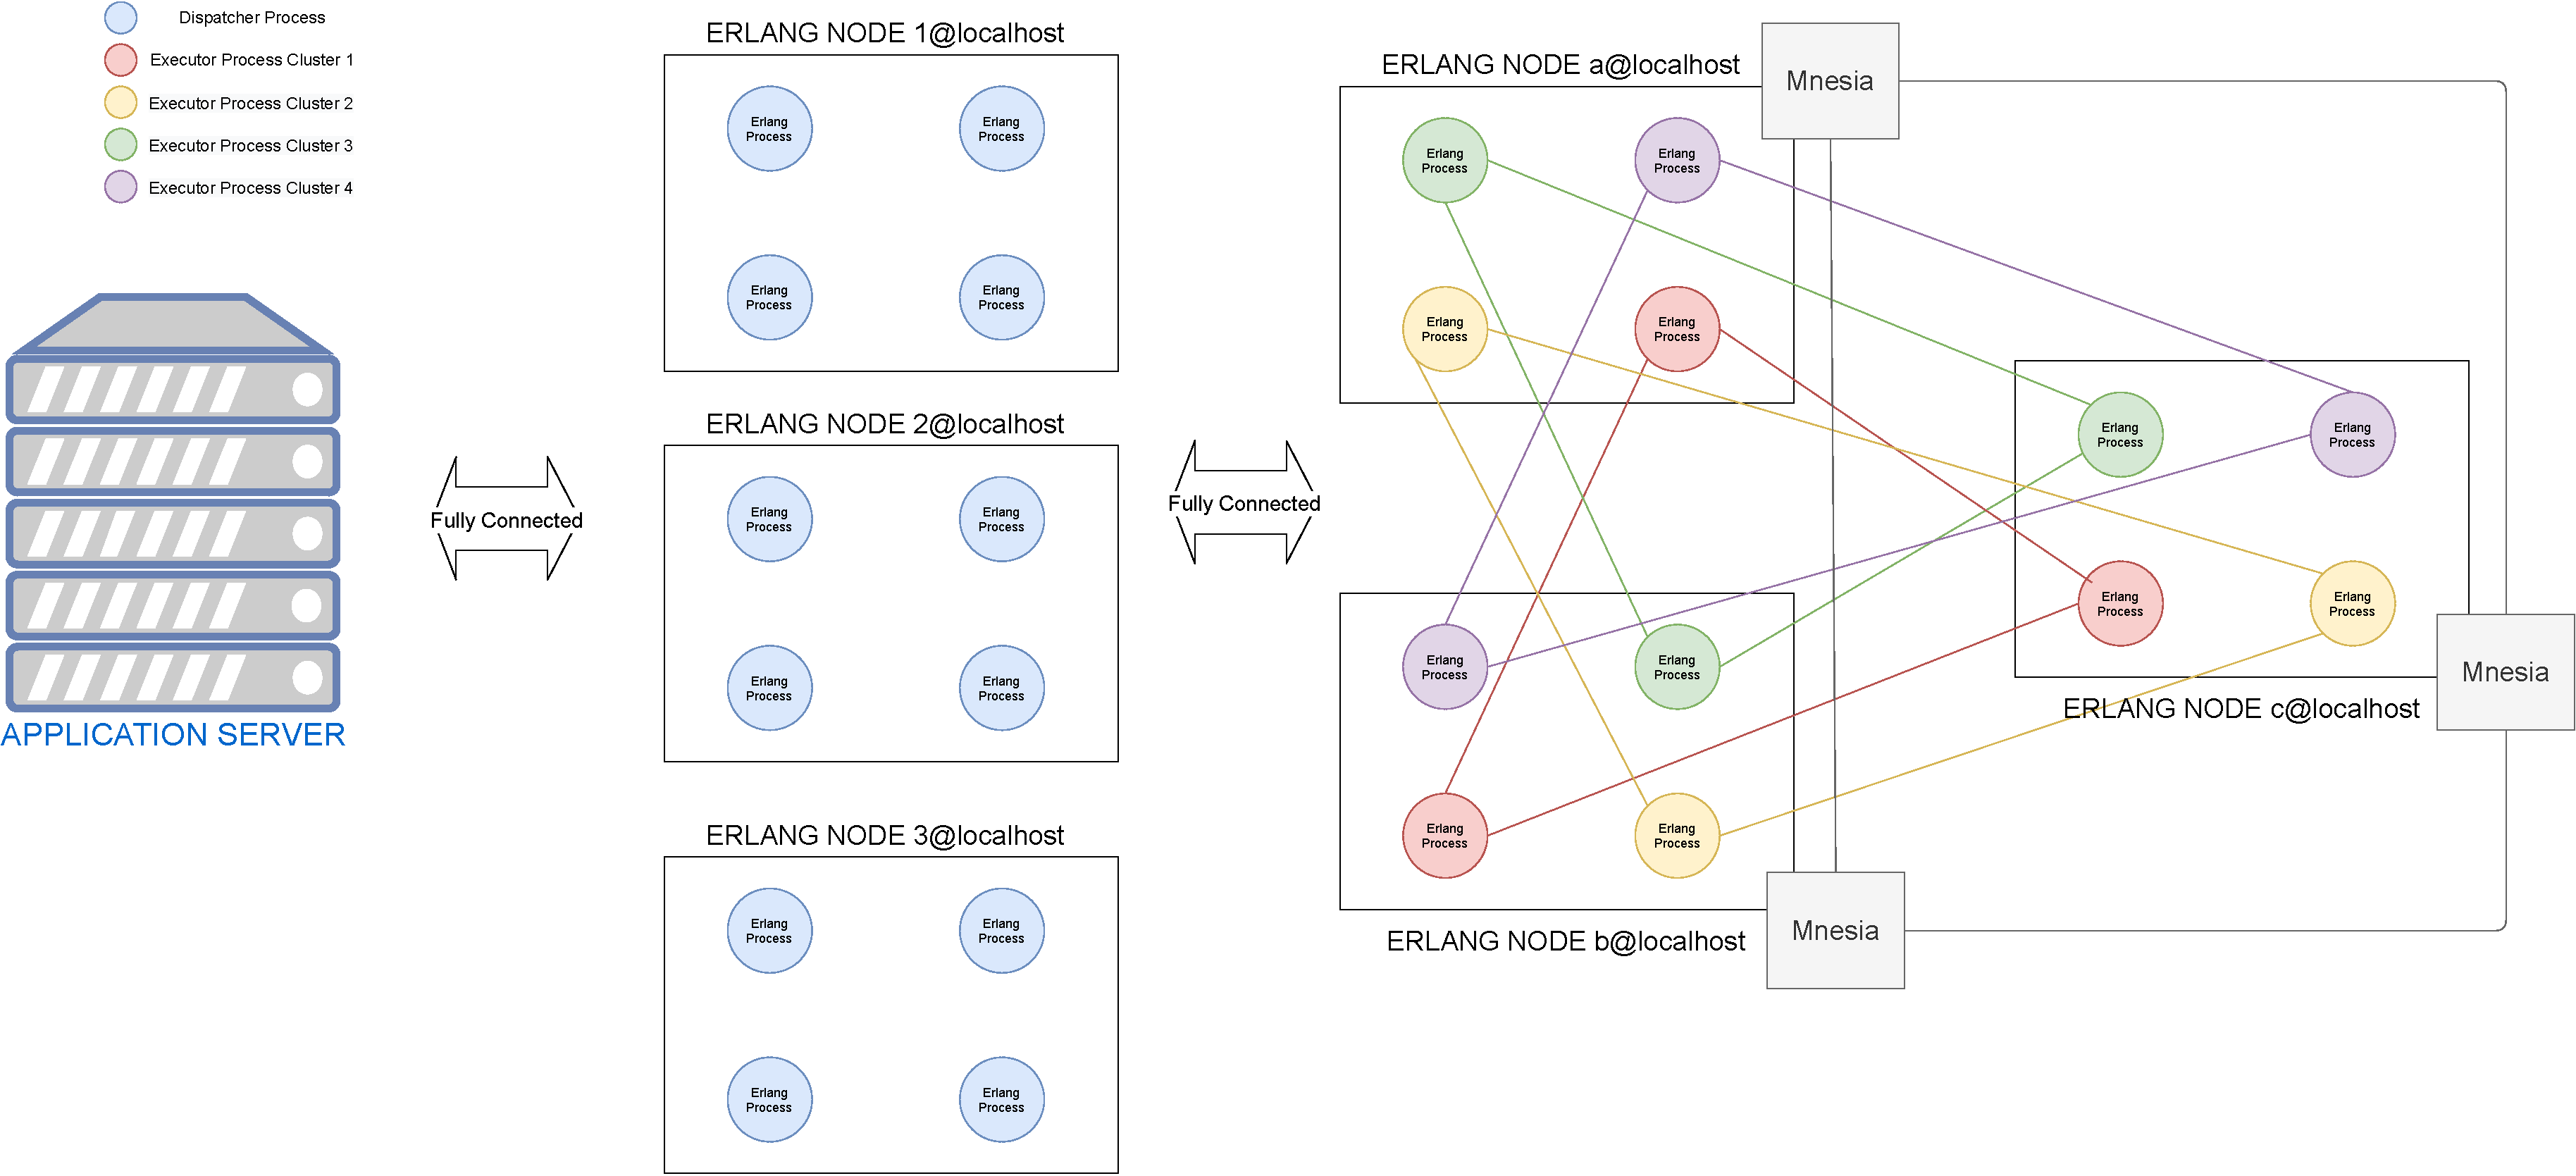
\includegraphics[width=\textwidth]{erlang_arch2}
	\caption{Erlang Subystem architecture.}\label{fig:erlang_arch2}
\end{figure}

\subsubsection{Dispatchers}

As can be seen from the architecture, multiple dispatcher instances are executed
on different dispatcher erlang nodes to allow the application server to always
find an available dispatcher in case a dispatcher process / dispatcher node
fails. Furthermore, the presence of multiple dispatcher instances allows the
application server to implement load-balancing techniques to balance the load of
requests between the dispatchers available;

\subsubsection{Executor Clusters}

Each Executor Cluster is organized according to a \textbf{leader-slaves
structure}. The leader manages the requests coming from the dispatchers,
communicate (if needed) to the Mnesia for the persistence of data, and calculate
the current AuctionState of the auctions and then sends it to the slaves. The
slaves have the function of replicas.

If the leader fails, the slaves will start a leader election process using the
\textbf{Bully algorithm}, to allow the cluster to remain operational.

\figref{fig:bully_state} shows the Bully algorithm state machine implemented in
this application.

\begin{figure}[h]
	\centering
	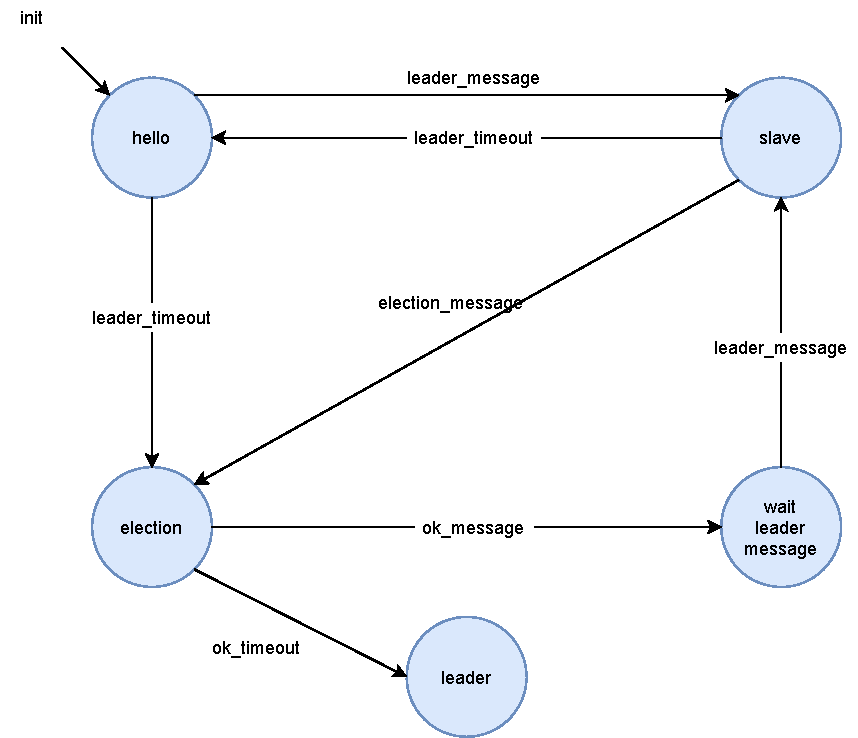
\includegraphics[width=\textwidth]{bully_state}
	\caption{Bully Algorithm State Machine}\label{fig:bully_state}
\end{figure}


Furthermore, as is visible from the architecture, the processes of each Executor
Cluster are executed in different executor erlang nodes (even if it is possible
that the same node executes more processes of the same cluster) so that the
clusters continue their operation even in case of failure of an executor erlang
node.
